\documentclass[tikz, border=3mm]{standalone}
\usepackage{tikz}
\usetikzlibrary{arrows.meta, decorations.markings, positioning}

\begin{document}
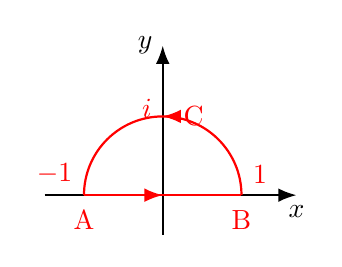
\begin{tikzpicture}[
    >=Latex, % Set default arrow tip style
    path/.style={red, thick}, % Style for the path
    arrow/.style={decoration={markings, mark=at position #1 with {\arrow{>}}}, postaction={decorate}}, % Style for arrows on path
    labelstyle/.style={red} % Style for labels
]

    % Axes
    \draw[->, thick] (-1.5, 0) -- (1.7, 0) node[below] {$x$};
    \draw[->, thick] (0, -0.5) -- (0, 1.9) node[left] {$y$};

    % Define key points
    \coordinate (A) at (-1, 0);
    \coordinate (B) at (1, 0);
    \coordinate (C) at (0, 1); % Top of the arc

    % Draw straight path segment A -> B with arrow
    \draw[path, arrow=0.5] (A) -- (B);

    % Draw arc path segment B -> A with arrow
    % The arc starts at angle 0, ends at angle 180, radius 1
    \draw[path, arrow=0.5] (B) arc (0:180:1);

    % Add labels for points A, B, C
    \node[labelstyle, below=2pt of A] {A};
    \node[labelstyle, below=2pt of B] {B};
    \node[labelstyle, right=4pt of C] {C};

    % Add labels for values -1, 1, i
    \node[labelstyle, above left=1pt of A] {$-1$};
    \node[labelstyle, above right=1pt of B] {$1$};
    \node[labelstyle] at (-0.2, 1.1) {$i$};

\end{tikzpicture}
\end{document}